\documentclass[12pt, xcolor=dvipsnames,svgnames,x11names]{article}
\usepackage{xcolor}
\usepackage{xspace}
\usepackage{url}
\usepackage[colorlinks=true,bookmarks=false,linkcolor=black,urlcolor=blue,citecolor=black]{hyperref}
\usepackage{fancyhdr}
\usepackage[top=1in,bottom=1.2in,left=1in,right=1in]{geometry}
\usepackage{multicol}
\usepackage{pgfplots}
\usepackage{tikz}
\usetikzlibrary{circuits.logic.US, patterns}
\usepackage{mathpazo}
\usepackage{biolinum} 
\usepackage[all]{tcolorbox}
\usepackage{derivative}
\usepackage{../Lectures/rahul_math}
\renewcommand{\familydefault}{\sfdefault}

% --- Custom Color Palette from Image ---
\definecolor{headerRed}{HTML}{A3403D} % Dark red from image top
\definecolor{patternBg}{HTML}{F2D9D7} % Light pinkish bg from image bottom
\definecolor{binaryText}{HTML}{D1A7A4} % Muted color for binary digits

% --- Background Pattern Setup ---
\usepackage[pages=all]{background}
\backgroundsetup{
scale=1,
color=black,
opacity=1,
angle=0,
contents={%
  \begin{tikzpicture}[remember picture,overlay]
    % Top Header Bar
    \fill[headerRed] (current page.north west) rectangle ([yshift=-1.2cm]current page.north east);
    % Bottom Binary Background
    \fill[patternBg] (current page.south west) rectangle ([yshift=3.5cm]current page.south east);
    % Decorative Line (from image)
    \draw[headerRed, line width=2pt] ([xshift=1in, yshift=-2.5cm]current page.north west) -- ([xshift=8in, yshift=-2.5cm]current page.north west);
    % Binary Text Overlay (Sample)
    \node[anchor=south, binaryText, font=\ttfamily\scriptsize, inner sep=0pt, yshift=1.5cm] at (current page.south) {
        \begin{tabular}{c@{\hspace{0.5em}}c@{\hspace{0.5em}}c@{\hspace{0.5em}}c@{\hspace{0.5em}}c@{\hspace{0.5em}}c@{\hspace{0.5em}}c}
        0 0 0 0 1 1 1 1 0 0 0 0 1 1 0 1 1 1 0 0 0 1 \\
        1 0 0 1 0 1 0 0 0 1 0 0 1 1 0 0 1 0 1 1 \\
        0 0 1 1 0 0 1 0 1 1 1 0 1 1 0 1 0 1 0 0 0 \\
        \end{tabular}
    };
  \end{tikzpicture}
}
}

\usetikzlibrary{positioning, arrows.meta, shadows}

% --- Header Styling ---
\makeatletter
\renewcommand{\maketitle}{%
    \vspace*{0.2cm}
    \begin{center}
        \begin{tcolorbox}[
            enhanced,
            colback=white,
            colframe=headerRed,
            arc=0mm,
            title={\textcolor{white}{\bfseries \@title}},
            coltitle=white,
            fonttitle=\bfseries\large,
            attach boxed title to top left={xshift=10pt, yshift=-\tcboxedtitleheight/2},
            boxed title style={sharp corners, colback=headerRed, frame hidden}
        ]
        \large
        \vspace{10pt}
        \noindent \textbf{Student Name:} \underline{\hspace{7cm}} \hfill \textbf{Points:} 30
        
        \vspace{10pt}
        \noindent \textbf{A Number:} \hfill \underline{\hspace{7cm}} \hfill \textbf{Due:} Feb 12, 2026
        \end{tcolorbox}
    \end{center}
    \vspace{10pt}
}
\makeatother

\newcommand{\hw}{Classwork 02//Training a Neural Network}
\newcommand{\duedate}{Jan 22, 2026}

\pagestyle{fancy}
\fancyhf{}
\lhead{\small CPE 487/587, Spring 2026}
\rhead{\small \textit{\hw}}
\cfoot{\thepage}
\renewcommand{\headrulewidth}{0pt}

\usepackage{booktabs} % For professional lines


% Define a very light gray for the rows
\definecolor{tablegray}{gray}{0.95}

\begin{document}

\title{\hw}
\maketitle




\section{Neural Network}

Consider a Neural Network as follows: \hfill \textbf{(10 Points)}

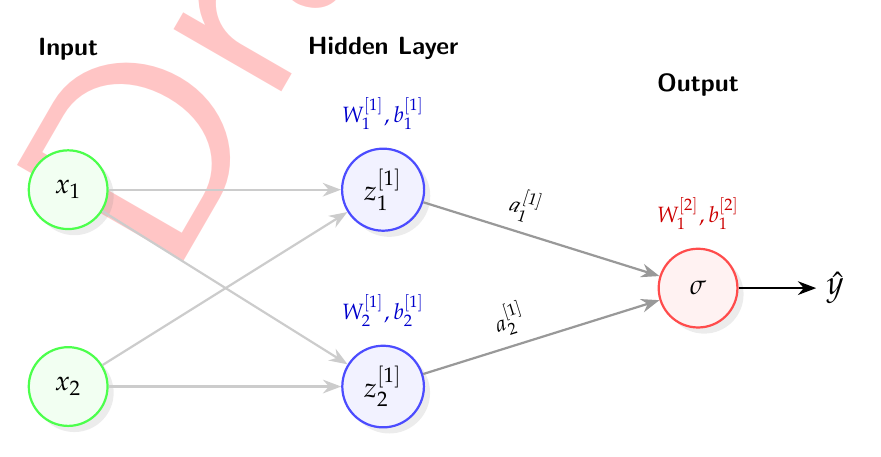
\begin{tikzpicture}[
    >=Stealth,
    node distance=2cm and 3cm,
    % Neurons
    neuron/.style={
        circle, draw=blue!70, fill=blue!5, thick, 
        minimum size=1cm, drop shadow={opacity=0.15}
    },
    input/.style={
        circle, draw=green!70, fill=green!5, thick, 
        minimum size=1cm, drop shadow={opacity=0.15}
    },
    output/.style={
        circle, draw=red!70, fill=red!5, thick, 
        minimum size=1cm, drop shadow={opacity=0.15}
    },
    % Labels
    label_text/.style={font=\small\bfseries},
    math_text/.style={font=\footnotesize}
]

    % --- CONFIGURATION: Change these to scale ---
    \def\numInput{2}
    \def\numHidden{2} % Change this to 3 or 4 to add more weights/nodes

    % --- INPUT LAYER ---
    \foreach \i in {1,...,\numInput} {
        \node[input] (I-\i) at (0, -\i*2.5) {$x_{\i}$};
    }

    % --- HIDDEN LAYER ---
    \foreach \j in {1,...,\numHidden} {
        \node[neuron] (H-\j) at (4, -\j*2.5) {$z_{\j}^{[1]}$};
        
        % Weights and Biases ABOVE the node
        \node[above=0.1cm of H-\j, math_text, blue!80!black] 
            {$W_{\j}^{[1]}, b_{\j}^{[1]}$};
    }

    % --- OUTPUT LAYER ---
    \node[output] (O) at (8, -3.75) {$\sigma$};
    \node[above=0.1cm of O, math_text, red!80!black] 
        {$W_{1}^{[2]}, b_{1}^{[2]}$};

    % --- CONNECTIONS ---
    % Input to Hidden
    \foreach \i in {1,...,\numInput} {
        \foreach \j in {1,...,\numHidden} {
            \draw[->, thick, gray!40] (I-\i) -- (H-\j);
        }
    }

    % Hidden to Output (with 'a' annotations)
    \foreach \j in {1,...,\numHidden} {
        \draw[->, thick, gray!80] (H-\j) -- (O) 
            node [pos=0.4, above, sloped, math_text, black] {$a_{\j}^{[1]}$};
    }

    % Final Output
    \draw[->, thick] (O) -- ++(1.5,0) node[right, font=\large] {$\hat{y}$};

    % --- LAYER TITLES ---
    \node[label_text, above=1cm of I-1] {Input};
    \node[label_text, above=1cm of H-1] {Hidden Layer};
    \node[label_text, above=1.8cm of O] {Output};

\end{tikzpicture}

We consider two features as input, with each neuron having Leaky ReLU as activation layer with negative slope coefficient $\alpha = 0.01$.

Consider the initial weights as

\begin{enumerate}
\item $W_1^{[1]} = [0.1, -0.2]$, and $b_1^{[1]} = 0.1$
\item $W_2^{[1]} = [0.2, 0.1]$, and $b_2^{[1]} = 0.2$
\item $W_1^{[2]} = [-0.3, 0.1]$, and $b_1^{[2jj]} = 0.1$.

\end{enumerate}

Given the input sample as $ \xbf = \{0.2, 0.1\}$ and known response variable as $y = x_1 + x_2 = 0.3$ what is the predicted $\yhat$. What is the squared error from the resulting network operation? Show your work.


\subsection{Solution}

\begin{align*}
z_1^{[1]} & = 0.2 \times 0.1 - 0.2\times 0.1 + 0.1 = 0.1\\
z_2^{[1]} & = 0.2 \times 0.2 + 0.1 \times 0.1 + 0.2 = 0.25\\
\end{align*}

Since we are using LeakyRELU, and $z_1^{[1]} > 0$, $z_2 {[1]} > 0$, $a_1^{[1]} = 0.1$, $a_2 {[1]} = 0.25$.

\begin{align*}
z_1^{[2]} = 0.1 \times -0.3 + 0.25 \times 0.1 + 0.1 = 0.095 = a_1^{[2]} = \hat{y}
\end{align*}

Squared error: $(0.3 - 0.095)^2 = 0.042025$.




\section{Early Stopping} We train a neural network with early stopping (patience = 2 which means stop if validation loss does not improve for 2 consecutive epochs). The loss values across 8 epochs are: \hfill \textbf{(10 Points)}

\begin{table}[h]
    \centering
    \caption{Neural Network Training and Validation Loss per Epoch}
    \label{tab:loss_history}
    \vspace{10pt}
  
    \begin{tabular}{ccc}
        \toprule
        \textbf{Epoch} & \textbf{Training Loss} & \textbf{Validation Loss} \\
        \midrule
        1 & 2.5 & 2.4 \\
        2 & 2.2 & 2.1 \\
        3 & 1.9 & 1.8 \\
        4 & 1.7 & 1.7 \\
        5 & 1.5 & 1.8 \\
        6 & 1.3 & 1.9 \\
        7 & 1.1 & 1.9 \\
        8 & 1.0 & 2.0 \\
        \bottomrule
    \end{tabular}
\end{table}

\begin{enumerate}
\item At which epoch do we trigger early stopping?
\item Which epoch’s model do we keep (the \textbf{best} model)?
\end{enumerate}

\subsection{Solution}

\begin{enumerate}
\item After epoch 6, we trigger early stopping

\begin{table}[h]
    \centering
    \label{tab:early_stopping}
    \begin{tabular}{|c|c|c|c|c|c|}
        \hline
        \textbf{Epoch} & \textbf{Val Loss} & \textbf{Best So Far} & \textbf{Improved?} & \textbf{Patience Counter} & \textbf{Action} \\
        \hline
        1 & 2.4 & 2.4 & Yes (init) & 0 & Continue \\
        \hline
        2 & 2.1 & 2.1 & Yes & 0 & Continue \\
        \hline
        3 & 1.8 & 1.8 & Yes & 0 & Continue \\
        \hline
        4 & 1.7 & 1.7 & Yes & 0 & Continue \\
        \hline
        5 & 1.8 & 1.7 & \textbf{No} & 1 & Continue \\
        \hline
        6 & 1.9 & 1.7 & \textbf{No} & 2 & \textbf{STOP} \\
        \hline
    \end{tabular}
\end{table}

\item From the previous table, it is clearer the model trained after the completion of Epoch 4 is the best model that we should keep.
\end{enumerate}

\section{Learning Rate Scheduler}

We use a step decay scheduler with: \hfill \textbf{(10 Points)}

\begin{enumerate}
\item Initial learning rate $\eta_0 = 0.1$
\item Decay rate $\gamma = 0.5$
\item Step size $s = 3$, i.e. learning rate decays after every three steps.
\end{enumerate}

Based on the above description, 

\begin{enumerate}
\item write down the formula for step decay learning rate $\eta(t)$ as a function of epoch $t$ and should be parametrized by $\eta_0$, $\gamma$ and $s$.
\item Calculate $\eta(t)$ for epoch $t=4$, $t = 7$, and $t = 9$.
\end{enumerate}


\subsection{Solution}

\begin{enumerate}

\item 

\begin{align*}
\eta(t) = \eta_0\gamma^{\lfloor \tfrac{t}{s} \rfloor}
\end{align*}
where $ \lfloor  \rfloor $ is the floor function.

\item Putting the values in the formula

\begin{align*}
\eta(t) & = \eta_0\gamma^{\lfloor \tfrac{t}{s} \rfloor}\\
\eta(4) & = 0.1 \times 0.5 ^{\lfloor \tfrac{4}{3} \rfloor} =0.05\\
\eta(7) & = 0.1 \times 0.5 ^{\lfloor \tfrac{7}{3} \rfloor} = 0.025\\
\eta(9) & = 0.1 \times 0.5 ^{\lfloor \tfrac{9}{3} \rfloor} = 0.0125
\end{align*}


\end{enumerate}

\end{document}